\documentclass[landscape,20pt]{extarticle}
\usepackage[utf8]{inputenc}
\usepackage[T1]{fontenc}
\usepackage[margin=2cm]{geometry}
\usepackage[parfill]{parskip}
\usepackage[pdftex]{graphicx}
\usepackage{amsmath}
%\usepackage[compact]{titlesec}

%\usepackage[sc]{mathpazo}
%\linespread{1.05}         % Palatino needs more leading (space between lines)

\renewcommand{\familydefault}{\sfdefault}
%\renewcommand*\rmdefault{cmfib}

\newcommand*{\TitleFont}{\Huge \bf}

\newcommand*{\TextFont}{\normalsize \it}

\begin{document}
\thispagestyle{empty}
\Large
{\TitleFont Introduction}

\begin{itemize}
\item The value of an Opinion\\
{\TextFont There a lot of different things one can use an opinion for.}
\item Analyzing Communication\\
{\TextFont Communication reflects an opinion.}
\item Semantic Orientation\\
{\TextFont Detecting if an opinion is negative or positive.}
\item Classifying tweets and counting them = opinion?\\
{\TextFont Is there a better way to extract an opinion?}
\item The ``influence'' of a tweet\\
{\TextFont Take followers, re-tweets and favorites into account!}
\end{itemize}

\newpage
\thispagestyle{empty}
\mbox{}

\clearpage
\thispagestyle{empty}

{\TitleFont System Overview}
\vspace{0.4cm}
\begin{center}
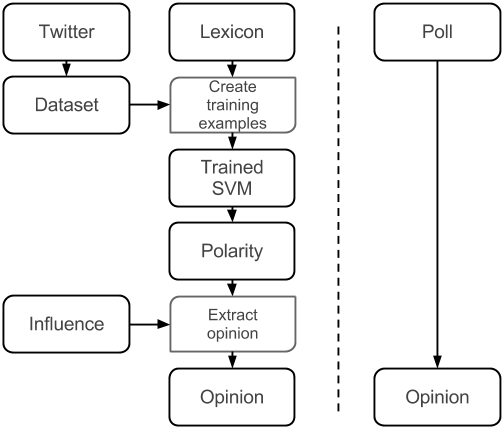
\includegraphics[scale=1]{../img/Overview.png}
\end{center}

\newpage
\thispagestyle{empty}
\mbox{}

\clearpage
\thispagestyle{empty}

{\TitleFont Method}

\begin{itemize}
\item The opinion of a brand, negative or positive?\\
{\TextFont To keep it simple we measured if the opinion was positive or negative.}
\item Opinion = position in a range\\
{\TextFont Essentially a score in the [0-100] range where 0 is fully negative.}
\item Must still classify tweets using the text alone\\
{\TextFont To use the influence one must know the initial opinion of the brand in the tweet.}
\item SVM + Supervised Learning through Lexicons\\
{\TextFont We used a SVM to classify, and the lexicons to make training data for the SVM.}
\item Evaluate the Lexicon, the SVM and the final algorithm\\
{\TextFont To make sure the different components yielded reasonable results we have to \\evaluate them, we used manual classification and a Poll to evaluate them.}
\end{itemize}

\newpage
\thispagestyle{empty}
\mbox{}

\clearpage
\thispagestyle{empty}

{\TitleFont Lexicon \& SVM}

\begin{itemize}
\item We use 7 different lexicons\\
{\TextFont Together they contain ca 8000 unique words with positive and negative scores.}
\item For each tweet we sum the scores of its words\\
{\TextFont Our pre-processing removes punctuation and lemmatize words for better results.}
\item From this score, we generate training data\\
{\TextFont Positive tweets are the \textit{n} with highest positive score, similarly for negative.\\
The neutral tweets are the \textit{n} longest tweets with a score of 0.}
\item The SVM represents the tweets using features\\
{\TextFont The features are unigrams and bigrams extracted from the pre-processed text.}
\item We make train the SVM with the generated training data\\
{\TextFont We then have a classifier for tweets about a brand which train automatically.}
\end{itemize}

\newpage
\thispagestyle{empty}
\mbox{}

\clearpage
\thispagestyle{empty}

{\TitleFont Algorithm}
\begin{itemize}
\item The influence of a tweet is computed using the number of Followers $Fo_t$ of the author, the number of Re-tweets $R_t$ and the number of Favorites $Fa_t$.
\begin{equation}
I_t = \log (Fo_t + 1) + R_t + Fa_t
\end{equation}

\item The opinion is computed as a percentage and aggregates the polarity of each tweet weighted by its influence.

\begin{equation}
Opinion = 100 \times \frac{\sum_{\substack{t \in T_{pos}}} I_t}{\sum_{\substack{t \in T_{pos}}} I_t + \sum_{\substack{t \in T_{neg}}} I_t}
\end{equation}

\end{itemize}

\newpage
\thispagestyle{empty}
\mbox{}

\clearpage
\thispagestyle{empty}

{\TitleFont Results}
\newline
\small{Manual classification}
\newline
\newline
\newline
\newline
\centerline{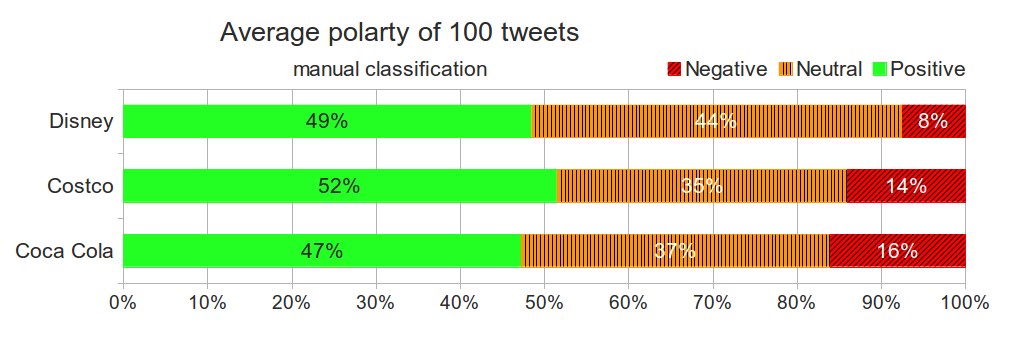
\includegraphics[scale=0.85]{../img/man1.png}}

\newpage
\thispagestyle{empty}
\mbox{}

\clearpage
\thispagestyle{empty}

{\TitleFont Results}
\newline
\small{Polarity scores}
\newline
\centerline{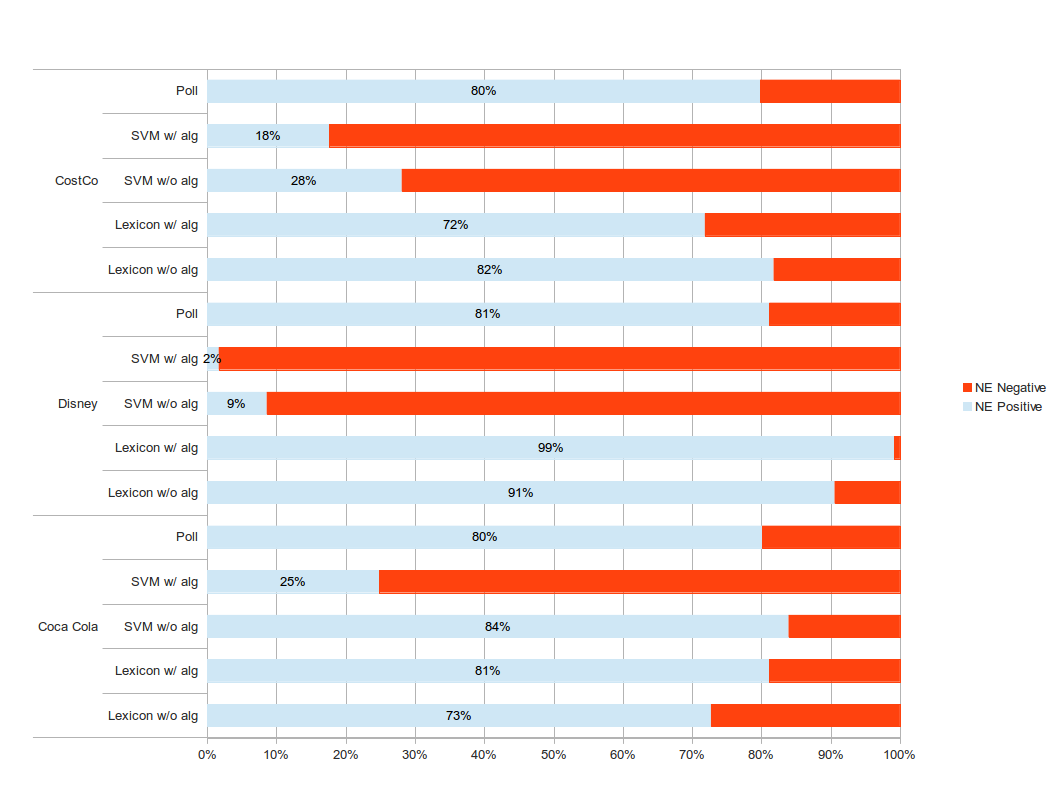
\includegraphics[scale=0.7]{../img/full1.png}}


\newpage
\thispagestyle{empty}
\mbox{}

\clearpage
\thispagestyle{empty}

{\TitleFont Discussion \& Conclusion}
\Large
\begin{itemize}
\item Tweets are notoriously hard to classify\\
{\TextFont Limited word-limit forces people to be very succint.}
\item Lexicons had a neutrality-bias\\
{\TextFont Could not quite identify the relevant parts}
\item The SVM had major problems\\
{\TextFont More features were needed, less noisy training data.}
\item The Algorithm actually made the result worse\\
{\TextFont At least one of the assumptions about Twitter users must be incorrect.}
\item Re-tweets dominate the influence\\
{\TextFont Since the algorithm made the result worse this may mean that people usually re-tweet tweets that they do not agree with.}
\end{itemize}

\end{document}
